\begin{itemize}
\item \textbf{Náhodný pokus} -- děj, jehož výsledek není předem jednoznačně určen podmínkami, za nichž probíhá.
\item \textbf{Náhodný jev} -- tvrzení o výsledku náhodného pokusu, přičemž o pravdivosti tohoto tvrzení lze po ukončení pokusu rozhodnout.
Náhodná veličina \uv{NV} -- \textbf{číselné} vyjádření výsledku náhodného pokusu.
\end{itemize}

\subsection{Náhodná veličina}
\begin{itemize}
	\item \textbf{Funkce}, která \textbf{každému elementárnímu jevu} $\omega \in \Omega$ \textbf{přiřadí reálné číslo} (převádí elementární jevy (abstraktní objekty) na čísla).
	\item Obvykle značíme velkými písmeny.
	\item \textbf{Hodnota} $X(\omega)$ \textbf{NV X závisí} na tom, který \textbf{elementární jev} $\omega$ \textbf{nastal} $\rightarrow$ víme-li, který elementární jev $\omega$ nastal, známe hodnotu $X(\omega)$ NV X.
\end{itemize}
\subsubsection*{Příklady}
\begin{itemize}
	\item[]	\begin{center}
		$X$... číselný výsledek hodu kostkou\\
		\end{center}
		\textbf{Náhodný pokus}: Hod kostkou. \\
		\textbf{Náhodný jev}: Padne sudé číslo. ($X \in \{2;4;6\}$) \\\\
		
	\item[]	\begin{center}
		$X$... rychlost připojení k internetu (Mb/s) \\
		\end{center}
		\textbf{Náhodný pokus}: Měření rychlosti připojení k internetu (download). \\
		\textbf{Náhodný jev}: Rychlost připojení k internetu je vyšší než 20 Mb/s.  ($X > 20$)\\\\
		
	\item[]	\begin{center}
		$X$... počet dívek mezi 1 000 náhodně vybranými dětmi \\
		\end{center}
		\textbf{Náhodný pokus}: Náhodný výběr 1 000 dětí a zjištění počtu dívek mezi nimi. \\
		\textbf{Náhodný jev}: Mezi 1 000 náhodně vybranými dětmi bude více než 500 dívek. ($X > 500$)
\end{itemize}





\subsection{Distribuční funkce F(x)}
\begin{itemize}
	\item Distribuční funkce F(t) udává pravděpodobnost, že náhodná veličina X bude \textbf{menší než} dané reálné číslo $t$. 
	$$F(t) = P(X <t)$$
	\item Distribuční funkce jednoznačně určuje rozdělení NV, tj. známe--li distribuční funkci, umíme určit pravděpodobnost $P(X \in M)$ pro libovolnou $M\subset \mathbb{R}$.
	\begin{figure}[H]
	\centering
	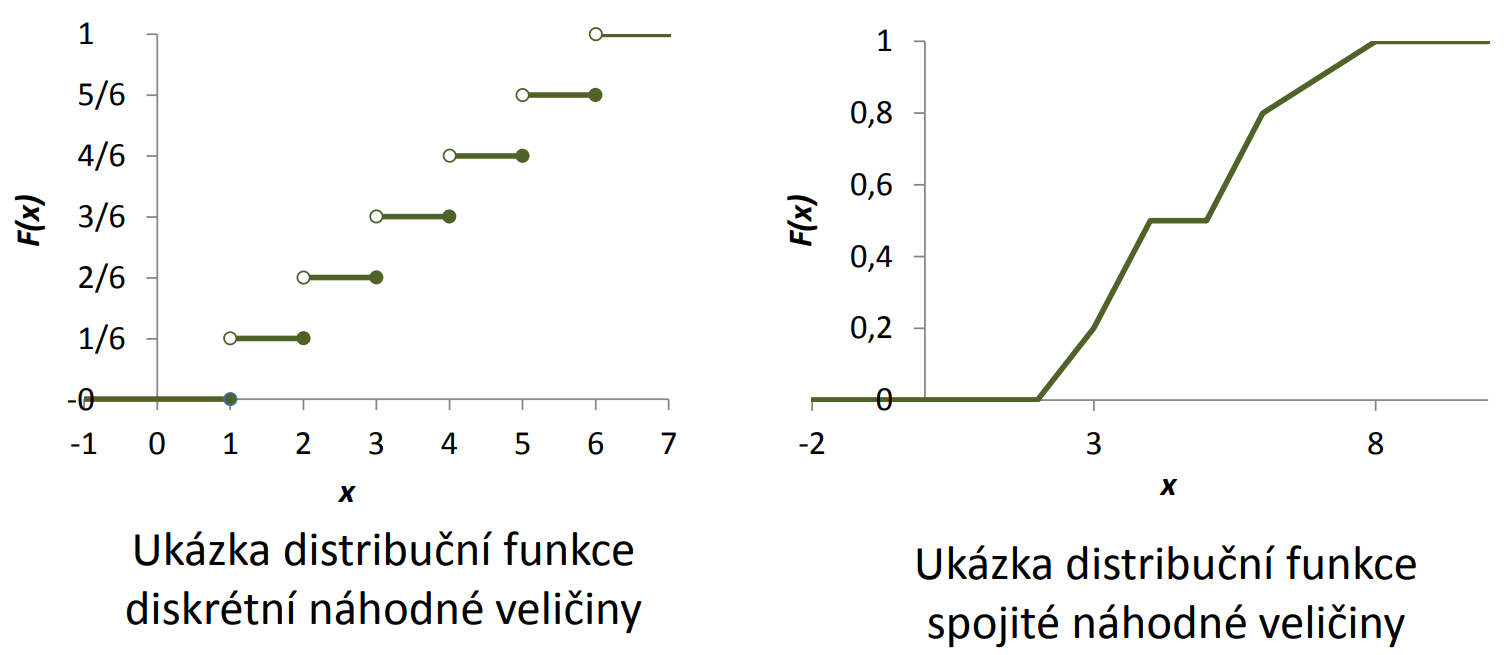
\includegraphics[width=0.75\textwidth]{assets/11_dist_fce}
	\end{figure}
\end{itemize}

\subsection{Základní typy náhodných veličin}
\begin{itemize}
	\item \textbf{Diskrétní NV} (nabývá spočetně mnoha hodnot)
	\item \textbf{Spojité NV} (jakákoliv hodnota na daném intervalu)
\end{itemize}

\subsection{Diskrétní náhodná veličina (\uv{DNV})}
\begin{itemize}
		\item Může \textbf{nabývat spočetně mnoha hodnot} (počet dní hospitalizace, počet dní nemocenské, počet zákazníků v lékárně během jednoho dne..).
		\item DNV X s distribuční funkcí $F_x(t)$ je charakterizována \textbf{Pravděpodobnostní funkcí} $P(X = x_i)$, tj. funkcí pro níž platí:
				\begin{equation*}
					F_x(t) = \sum_{x_i<t}P(X = x_i)= \sum_{x_i<t}P(x_i).
				\end{equation*}
\end{itemize}
\subsubsection{Pravděpodobnostní funkce}
			\begin{itemize}
				\item $P(x_i) \geq 0$
				\item $\sum_i P(X = x_i) = 1$
				\item Lze zadat předpisem, tabulkou, grafem.
				\begin{figure}[H]
					\centering
					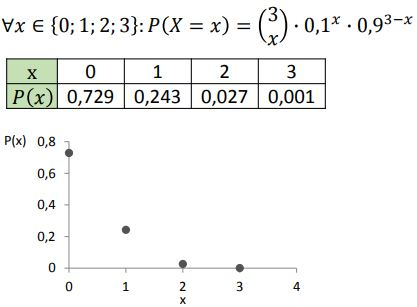
\includegraphics[width=0.6\textwidth]{assets/11_dnv_prav}
				\end{figure}
				\item[$\Rightarrow$] \textit{Příklad} -- Při ověřování kvality výroby jsou náhodně vybrány dva výrobky a je testována jejich kvalita. Počet vadných výrobků mezi vybranými modelujeme náhodnou veličino X. Z dlouhodobého pozorování jsou známy údaje uvedené v následující tabulce.
				\begin{table}[H]
					\centering
					\begin{tabular}{c|c}
						\textbf{Počet vadných výrobků}            & \textbf{Pravděpodobnost} \\\hhline
						0      &   0,25      \\ 
						1      &   0,50    \\
						2	   &   0,25
					\end{tabular}
				\end{table}
				\textit{Určete pravděpodobnostní a distribuční funkci počtu vadných výrobků v testovaném vzorku.}
				\begin{figure}[H]
					\centering
					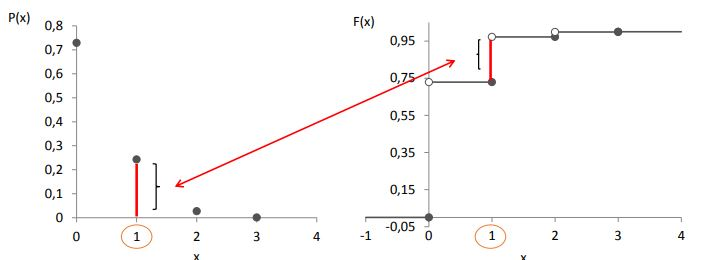
\includegraphics[width=0.75\textwidth]{assets/11_vztah_prav_dist_dnv}
				\end{figure}
				\item \textbf{Body nespojitosti} distribuční funkce jsou body, v nichž je pravděpodobnostní funkce nenulová.
				\item $P (X= a) = \lim_{x\to a+} F(x) - F(a)$ , tj. velikost \uv{skoku} distribuční funkce v bodech nespojitosti je rovna příslušným hodnotám pravděpodobnostní funkce.
			\end{itemize}
\subsubsection{Distribuční funkce}
				\begin{itemize}
					\item $F(t) = \sum_{x_i < t} P(x_i)$
					\item Lze zadat předpisem, tabulkou, grafem.
					\begin{figure}[H]
					\centering
					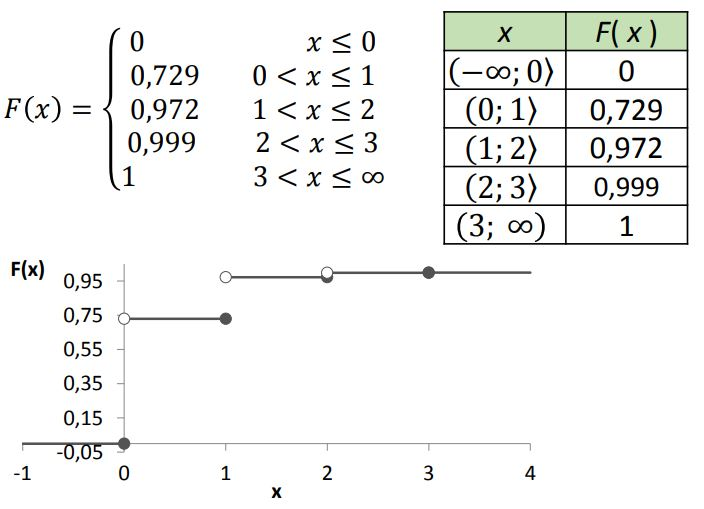
\includegraphics[width=0.6\textwidth]{assets/11_dnv_dist}
				\end{figure}
				\item Distribuční funkce $F(t)$ \textbf{udává pravděpodobnost}, že náhodná veličina $X$ bude \textbf{menší než} dané reálné číslo $t$. $$F(t) = P(X < t)$$
			\end{itemize}
\subsubsection*{Vlastnosti distribuční funkce}
				\begin{itemize}
					\item $0 \leq F(t) \leq 1$,
					\item je neklesající,
					\item je zleva spojitá,
					\item má nejvýše spočetně mnoho bodů nespojitosti,
					\item $F(t) \rightarrow 0 $ pro $ t \rightarrow -\infty $ (\uv{začíná} v 0),
					\item $F(t) \rightarrow 1 $ pro $ t \rightarrow \infty $ (\uv{končí} v 1).
				\end{itemize}
				\begin{figure}[H]
					\centering
					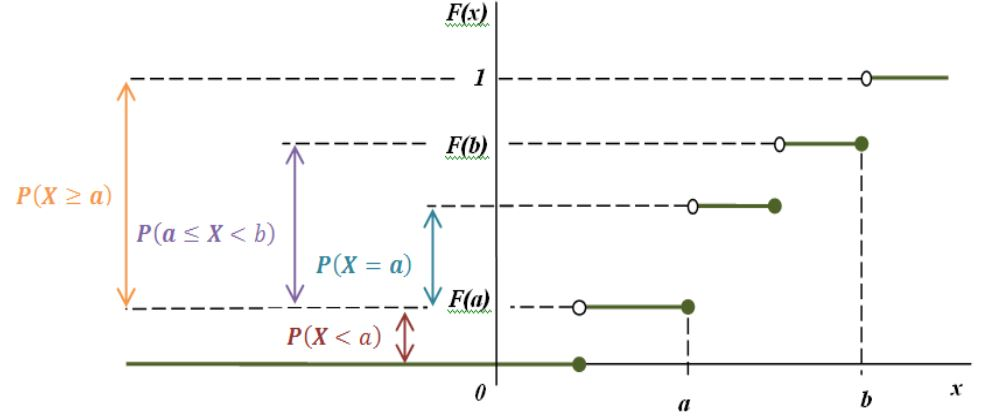
\includegraphics[width=0.75\textwidth]{assets/11_vztah_prav_dist_dnv2}
				\end{figure}
				$$P(X = a) \lim_{x \to a+} F(x) - F(a)$$

\subsection{Spojitá náhodná veličina (\uv{SNV})}

\begin{itemize}
		\item Náhodná veličina $X$ má spojité rozdělení pravděpodobnosti (zkráceně \uv{je spojitá}) právě když má spojitou distribuční funkci.
		\item Mohou \textbf{nabývat všech hodnot na nějakém intervalu} (mají spojitou distribuční funkci) (doba do remise onemocnění, výška, váha, BMO, IQ, vitální kapacita plic, chyba měření...).
		\item SNV X s distribuční funkcí $F_x(t)$ je charakterizována \textbf{hustotou pravděpodobností} $f(x)$, tj. funkcí pro níž platí:
		\begin{equation*}
				F_x(t) = \int_{-\infty}^{t} f(x) dx.
		\end{equation*}
	\end{itemize}
\subsubsection{Hustota pravděpodobnosti f(x)}
\begin{equation*}
F(x) = \int_{-\infty}^{t} f(x) dx \Rightarrow f(x) = \frac{dF}{dx}
\end{equation*}
\subsubsection*{Vlastnosti hustoty pravděpodobnosti}
\begin{itemize}
	\item $f(x)$ je reálná nezáporná funkce,
	\item $\int_{-\infty}{\infty} f(x) = 1$ (plocha pod křivkou hustoty je 1), 
	\item $\lim_{x \to -\infty} f(x) = 0$ (\uv{začíná v 0}),
	\item $\lim_{x \to \infty} f(x) = 0$ (\uv{končí v 0}).
	\begin{figure}[H]
		\centering
		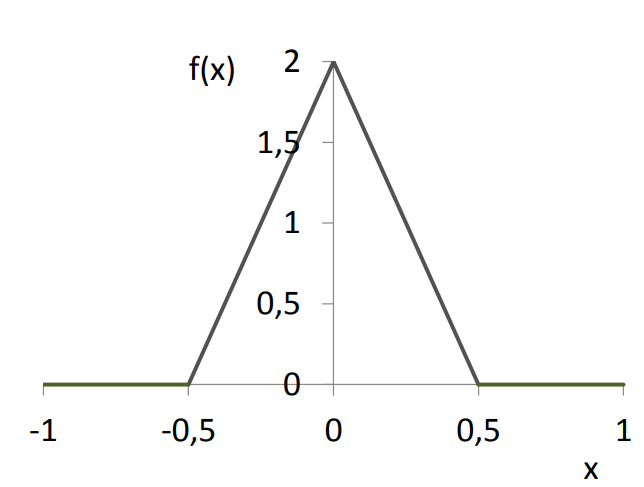
\includegraphics[width=0.35\textwidth]{assets/11_snv_muze}
		\caption{$f(x)$ může nabývat hodnot vyšších než 1}
	\end{figure}
\end{itemize}
\subsubsection{Distribuční funkce}
$$F_x(t) = \int_{-\infty}^{t} f(x) dx\, \quad P(X = a) = 0$$
\begin{figure}[H]
	\centering
	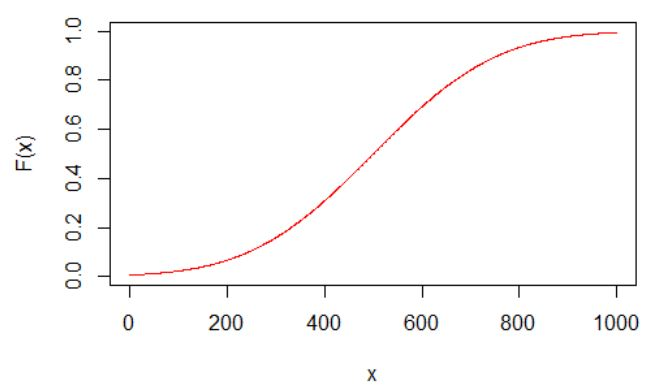
\includegraphics[width=0.5\textwidth]{assets/11_dist_fce_snv}
\end{figure}
\begin{figure}[H]
	\centering
	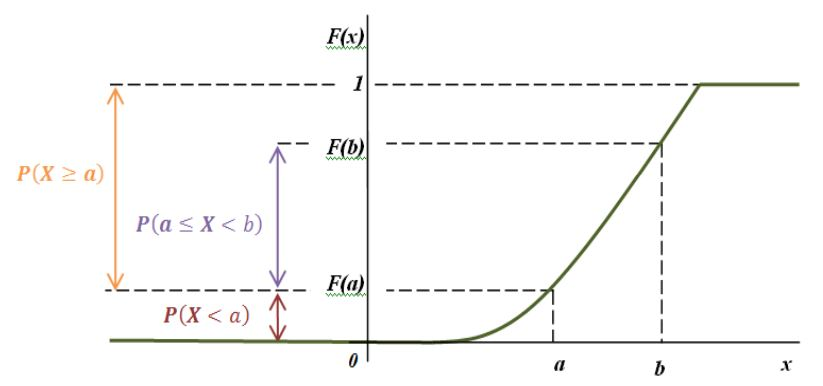
\includegraphics[width=0.6\textwidth]{assets/11_vztah_prav_dist_snv}
	\caption{Vztah mezi pravděpodobností a distribuční funkcí}
\end{figure}

\subsection{Číselné charakteristiky NV}
\begin{itemize}
	\item Distribuční funkce (pravděpodobnostní funkce, hustota pravděpodobnosti) popisují rozdělení NV jednoznačně, do všech podrobností. 
	\item Někdy nás zajímá pouze některý aspekt NV, který se dá popsat jedním číslem:
	\begin{itemize}
		\item očekávaná hodnota NV,
		\item variabilita možných hodnot,
		\item hodnota, pod níž leží pouze malé množství hodnot NV,
		\item šikmost rozdělení,
		\item koncentrace hodnot NV kolem očekávané hodnoty (špičatost rozdělení).\\

		\item \textbf{Obecný moment r--tého řádu} (značí se $\mu_r$ nebo $E(X^r)$, pro r=1,2...) \\pro diskrétní NV: $\qquad \mu_r = \sum_{(i)}x_i^r \cdot P(x_i)$ \\pro spojitou NV: $\qquad \mu_r = \int_{-\infty}^{\infty} x^r \cdot f(x) dx$
		\item \textbf{Střední hodnota} (expected value, mean, značí se jako $\mathbf{E(X)}$ nebo $\mu$) \\pro diskrétní NV: $\qquad E(X) = \mu = \sum_{(i)}x_i \cdot P(x_i)$\\pro spojitou NV: $\qquad E(X) = \mu = \int_{-\infty}^{\infty} x \cdot f(x)dx$
		\item \textbf{Centrální moment r--tého řádu} $\mathbf{\mu_r}$' (značíme $\mu_r$' $= E[(X - E(X))]^r$) \\pro diskrétní NV: $\qquad \mu_r' = \sum_{(i)}(x_i -E(X))^r \cdot P(x_i)$\\pro spojitou NV: $\qquad \mu_r' = \int_{-\infty}^{\infty} (x - E(X))^r \cdot f(x)dx$
		\item \textbf{Rozptyl} (dispersion, variance; značí se $\mu_2'$ nebo $DX$ nebo $\sigma^2$) \\pro diskrétní NV: $\qquad D(X) = \mu_2' = \sum_{(i)}(x_i -E(X))^2 \cdot P(x_i)$\\pro spojitou NV: $\qquad D(X) = \mu_2' = \int_{-\infty}^{\infty} (x - E(X))^2 \cdot f(x)dx$
	\end{itemize}
\end{itemize}

\subsubsection{Význam střední hodnoty}
Střední hodnotu $E(X)$ náhodné veličiny $X$ lze chápat jako:
\begin{itemize}
	\item průměrnou (očekávanou) hodnotu NV $X$, kolem níž hodnoty NV kolísají,
	\item míru polohy, populační průměr,
	\item vážený průměr všech možných hodnot ($E(X) = \sum_{(i)}x_i \cdot P(x_i)$),
	\item \uv{těžiště} možných hodnot.
	\begin{figure}[H]
			\centering
			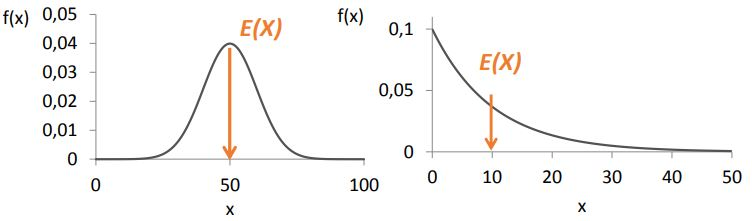
\includegraphics[width=0.7\textwidth]{assets/11_stredni_hodnota}
	\end{figure}
\end{itemize}

\subsubsection{Kvantily}
\textbf{p--kvantil} $\mathbf{x_p}$ (také $100_p\%$--ní kvantil je číslo, pro které platí): $$P(X < x_p) = p.$$ 
\begin{center}
$\Rightarrow F(x_p) = p \Rightarrow x_p = F^{-1}(p)$ \\
(tj. kvantilová funkce $F^{-1}(p)$ je funkcí inverzní k distribuční funkci $F(x_p)$)
\begin{figure}[H]
			\centering
			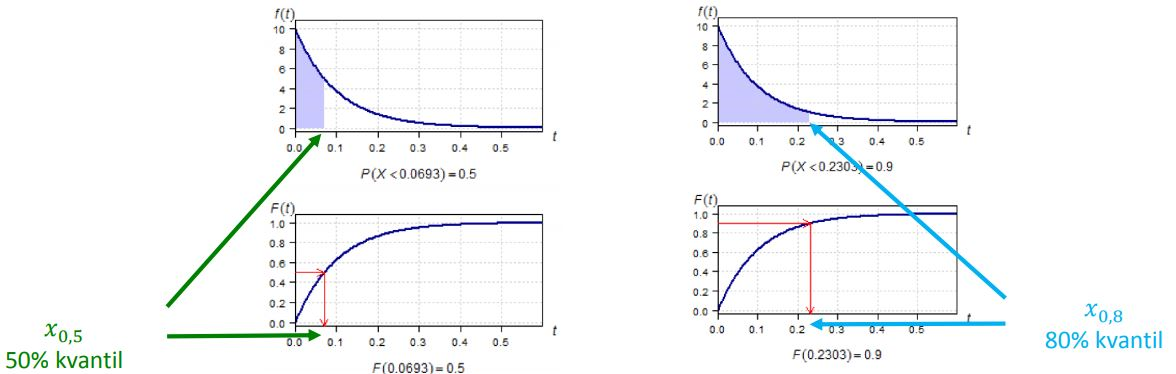
\includegraphics[width=0.9\textwidth]{assets/11_kvantily}
	\end{figure}
\end{center}

\noindent Kvantily obvykle určujeme \textbf{pouze pro SNV}. \textbf{Význačné kvantily}:
\begin{itemize}
	\item \textbf{Kvartily}
	\begin{itemize}
		\item[] Dolní kvartil $x_{0,25}$
		\item[] Medián $x_{0,5}$
		\item[] Horní kvartil $x_{0,75}$
	\end{itemize}
	\item \textbf{Decily} -- $x_{0,1}; x_{0,2}; ... ;x_{0,9}$
	\item \textbf{Percentily} -- $x_{0,01}; x_{0,02}; ... ;x_{0,99}$
	\item \textbf{Minimum} $x_{min}$ a \textbf{Maximum} $x_{max}$
\end{itemize}

\subsubsection{Modus}
\textbf{Modus} $\mathbf{\hat{x}}$ -- typická hodnota náhodné veličiny
\begin{itemize}
\item \textbf{pro diskrétní NV} -- $x_i: P(X = \hat{x}) \geq P(X = x_i)$ (tzn. modus je taková hodnota DNV, v níž $P(x_i)$ nabývá svého maxima).
\item \textbf{pro spojité NV} -- $ x_i: f(\hat{x}) \geq f(x)$ (tzn. modus je taková hodnota SNV, v níž $f(x)$ nabývá svého maxima).
	\item Modus není těmito podmínkami určen jednoznačně, tzn. náhodná veličina může mít několik modů (např. výsledek hodu kostkou). Má-li NV právě jeden modus, mluvíme o \textbf{unimodálním rozdělení NV}.
	\item Má-li NV unimodální symetrické rozdělení, pak $E(X) = x_{0,5} = \hat{x}$.
\end{itemize}

\subsubsection{Význam rozptylu}
\begin{itemize}
	\item \textbf{Míra variability dat kolem střední hodnoty}.
	\item Střední kvadratická odchylka od střední hodnoty ($D(X) = E(X - E(X))^2$).
	\item Malý rozptyl $\approx$ hodnoty NV se s vysokou pravděpodobností objevují blízko $E(X)$.
	\item Velký rozptyl $\approx$ hodnoty NV se často objevují ve velké vzdálenosti od $E(X)$.
	\item Jednotka rozptylu je kvadrátem jednotky náhodné veličiny.
	\begin{figure}[H]
			\centering
			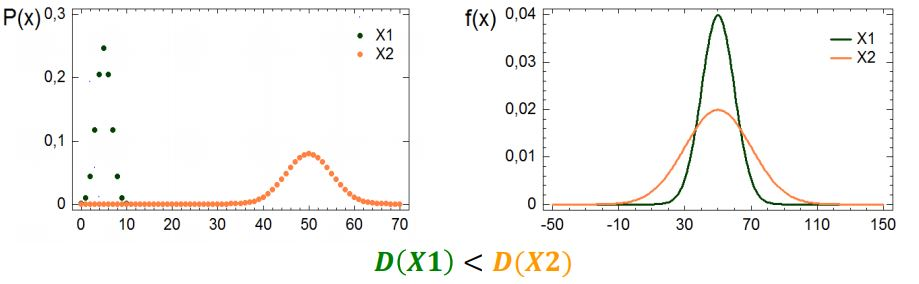
\includegraphics[width=0.9\textwidth]{assets/11_rozptyl}
	\end{figure}
\end{itemize}

\subsubsection{Směrodatná odchylka $\mathbf{\sigma}$}
$$\sigma(Y) = \sqrt{D(X)}$$
Jendá se o odmocninu rozptylu náhodné veličiny. Směrodatná odchylka \textbf{neumožňuje} srovnávat variabilitu náhodných veličin \textbf{měřených v různých jednotkách}! 

\subsubsection{Variační koeficient}
\textbf{Variační koeficient} $\mathbf{\gamma}$ je definován pouze pro \textbf{nezáporné} náhodné veličiny. $$\gamma = \frac{\sigma}{\mu'}, \textrm{ resp. } \frac{\sigma}{\mu'} \cdot 100 [\%]$$
\begin{itemize}
	\item Variační koeficient -- \textbf{směrodatná odchylka v procentech} střední hodnoty.
	\item Čím nižší var. koeficient, tím \textbf{homogennější} soubor.
	\item $V_X > 50\%$ značí silně rozptýlený soubor.
\end{itemize}